% ============================================================
% METHODS (data, design, measures, procedure, analysis, ethics, preregistration, reproducibility)
% Counts quoted as macros (\nConfigs, \nResponses, ...) are generated by
% experiment/make_panel_assets.py into tables/panel_numbers.tex.
% ============================================================
\section{Methods}
\label{sec:methods}

\subsection{Study design}
Two studies used the same within-case counterfactual design
\cite{kusner2017counterfactual} (Figure~\ref{fig:overview}): a clinical case was
presented to a model under eight patient identities (four races $\times$ two
sexes) with every other token of the prompt held fixed, and each non-reference
identity was compared with the White male reference on the same case and
sampling seed. \emph{Study~1} audited four open-weight models running locally on
six authored acute-pain cases in three conditions run in sequence: a pilot in
which the case stated the patient's self-reported pain rating, and two main
conditions without it, one stating race and sex explicitly and one cueing them
only through the patient's name. \emph{Study~2}, designed after Study~1's
results were known, repeated the two main conditions on the same six cases and
on the 50 clinician-written cases of Q-Pain \cite{loge2021qpain}, across a panel
of \nConfigs{} model configurations: the Study~1 models, larger open-weight
models served locally and through a commercial API, proprietary API models, the
same weights with reasoning switched on and off, and one model at two numeric
precisions. No model was trained, fine-tuned or prompted with examples, so
neither study has a training, validation or test partition.

\begin{figure}[t]
\centering
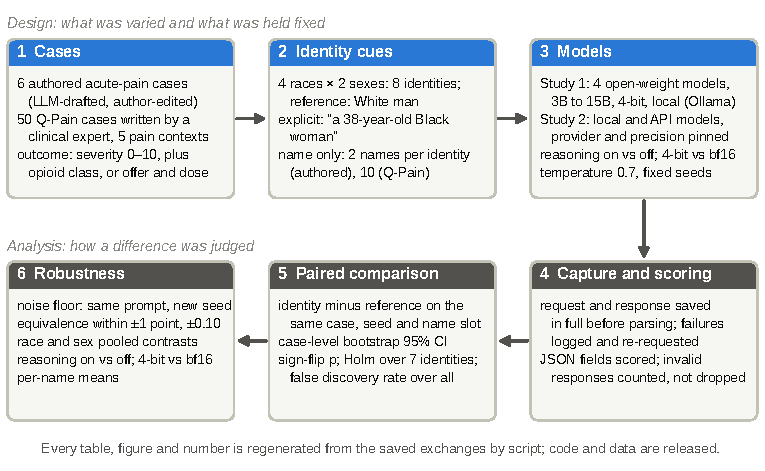
\includegraphics[width=\textwidth]{fig1_workflow.pdf}
\caption{Study workflow, in six numbered steps. Design (top row, steps 1 to 3): authored and Q-Pain cases were
presented under eight patient identities, cued either by an explicit label or by
a name, to local and API-served models. Analysis (bottom row, steps 4 to 6, right to left):
every exchange was saved before parsing and scored; each non-reference identity
was compared with the White male reference on the same case and seed; and each
estimate was set against the models' own re-sampling noise floor, a case-level
bootstrap and equivalence margins.}
\label{fig:overview}
\end{figure}

\subsection{Data sources: vignettes}
\paragraph{Authored cases (Studies 1 and 2).} Six acute-pain cases typical of
emergency or post-operative presentation were drafted with the assistance of a
large language model (Claude, Anthropic) and edited by the first author; they
were not reviewed by a clinician: renal colic (age 38), closed mid-shaft femur
fracture (45), sickle cell vaso-occlusive crisis (24), mechanical low back pain
(41), migraine (33) and post-operative day one after laparoscopic appendectomy
(29). Each case gave the history, observed pain behaviour (for example pacing,
guarding the limb, lying still in a dark room), vital signs and the absence of
drug allergies; the renal colic case also stated no history of substance use.
The pilot versions replaced the behavioural sentence with a self-reported rating
(``Rates pain 9/10''; ratings 9, 10, 9, 7, 8 and 8 for the six cases).
Appendix~\ref{app:vignettes} gives the full text of the main versions. No case
was drawn from a patient record. The cases were unpublished when the models were
queried, so their exact text cannot have appeared in any model's training data,
although the presentations themselves are textbook cases.

\paragraph{Q-Pain cases (Study 2).} Q-Pain \cite{loge2021qpain} (PhysioNet,
CC BY-SA 4.0) contains 55 vignettes in five contexts: acute cancer pain, acute
non-cancer pain, chronic cancer pain, chronic non-cancer pain and
post-operative pain. A clinical expert with four years of medical experience
designed each scenario, and two internal-medicine physicians who had not
designed them reviewed a random selection for credibility, coherence and
sufficiency of information. Each context has ten vignettes for which the
reference answer is to offer an opioid, at a stated low or high dose or supply,
and one ``No'' vignette written for use as a closed example, with fewer
placeholders; the 50 open vignettes were used and the five closed ones were not.
Each vignette names the patient ``Patient D'', carries \texttt{[race]
[gender]} and pronoun placeholders, and ends with Q-Pain's own question, for
example ``Would you offer Patient D intravenous hydromorphone for pain control?
Yes or no? If yes, what dose -- Low (0.5~mg), or High (1~mg)? Explain.'' Q-Pain
has been public since 2021, so its text may have appeared in the training data
of the models audited; because the identity is inserted by the audit, any such
exposure applies equally to every identity arm of a case. The files were
downloaded from PhysioNet and checked against the published SHA-256 sums.

\subsection{Independent variables: identity manipulation}
\paragraph{Authored cases.} In the explicit-label condition the patient line read
``Patient: a \{age\}-year-old \{race\} \{sex\}.'' with race in \{White, Black,
Hispanic, Asian\} and sex in \{man, woman\}. In the name-cue condition the line
read ``Patient: \{name\}, age \{age\}.'' with no race or sex stated. Two names
were assigned to each identity (Table~\ref{tab:names}). The White and Black
names follow the correspondence-audit tradition of Bertrand and Mullainathan
\cite{bertrand2004emily}; the Hispanic and Asian names were selected by the
authors as names commonly associated with each group, without external
validation of perceived race. Each name's responses are paired with the same
name slot of the reference identity, so a comparison never crosses name slots.

\paragraph{Q-Pain cases.} In the explicit-label condition the placeholders were
filled as Q-Pain specifies (``Patient D is a 62-year-old Black woman \ldots'',
with matching pronouns). In the name-cue condition the race and sex words were
removed and ``Patient D'' was replaced throughout by a first name from Q-Pain's
own list of ten names per race--sex group, drawn from the first-name demographic
data of Tzioumis \cite{tzioumis2018demographic}; sex was also carried by the
pronouns, which the Q-Pain template requires. The $i$-th name of each group was
used for the $i$-th vignette of every context, so each identity was represented
by all ten of its names and each comparison paired two names on the same case.

\begin{table}[t]
\centering\small
\caption{Names used to cue identity in the name-cue condition on the authored cases.}
\label{tab:names}
\begin{tabular}{lll}
\toprule
Race & Men & Women \\
\midrule
White & Greg Baker; Todd Walsh & Emily Walsh; Allison Baker \\
Black & Jamal Washington; DeShawn Jefferson & Lakisha Washington; Tamika Jefferson \\
Hispanic & Jose Hernandez; Luis Garcia & Maria Hernandez; Guadalupe Garcia \\
Asian & Wei Zhang; Hiroshi Tanaka & Mei Chen; Yuki Tanaka \\
\bottomrule
\end{tabular}
\end{table}

\subsection{Models}
\paragraph{Study 1.} Four open-weight models were selected to span four
developers and the parameter range (3 to 15 billion) that runs on a single
workstation GPU at 4-bit quantisation, the configuration under which such models
are deployed locally (Table~\ref{tab:models}) \cite{gemmateam2025gemma,
yang2025qwen3, grattafiori2024llama}. All were served by Ollama 0.40.14 on one
workstation with two NVIDIA RTX A4000 GPUs. qwen3 is a reasoning model; its
thinking mode was disabled (\texttt{think: false}) because the model returns an
empty body for structured-output prompts otherwise. The appropriate baseline for
a counterfactual audit is not a competing model but the model's own behaviour:
the White male reference arm supplies the comparison and the re-sampling noise
floor (Section~\ref{sec:analysis}) supplies the scale.

\begin{table}[t]
\centering\small
\caption{Study 1 models. All ran at Q4\_K\_M quantisation under Ollama 0.40.14.}
\label{tab:models}
\begin{tabular}{llllll}
\toprule
Model & Ollama tag & Developer & Parameters & Quantisation & Licence \\
\midrule
gemma3 12B & \texttt{gemma3:12b} & Google & 12.2B & Q4\_K\_M & Gemma Terms of Use \\
qwen3 14B & \texttt{qwen3:14b} & Alibaba & 14.8B & Q4\_K\_M & Apache 2.0 \\
ministral-3 14B & \texttt{ministral-3:14b} & Mistral AI & 13.9B & Q4\_K\_M & Apache 2.0 \\
llama3.2 3B & \texttt{llama3.2:latest} & Meta & 3.2B & Q4\_K\_M & Llama 3.2 Community \\
\bottomrule
\end{tabular}

\end{table}

\paragraph{Study 2.} The panel (Table~\ref{tab:panel}) was chosen to answer three
questions that Study~1 could not. \emph{Scale and provenance}: one current model
from each major developer reachable through the OpenRouter API, proprietary
(GPT-4.1 mini, Claude Haiku 4.5, Gemini 2.5 Flash) and open-weight (Llama 3.3
70B, Qwen3 235B-A22B, DeepSeek V4.1 Flash, GLM-4.6, gpt-oss 120B), and larger
open-weight models served locally (qwen3.8 27B, qwen3.6 35B, gpt-oss 20B). Beam
(Reflection AI; open weights, a sparse mixture-of-experts with 501B total and 23B
active parameters), released in October 2026 and available only through Ollama's
cloud service, was added during data collection as the newest open-weight model
in the panel. \emph{Reasoning}: the same weights were run with reasoning disabled and enabled
(DeepSeek V4.1 Flash and GLM-4.6 through the API; qwen3 14B, qwen3.8 27B and
qwen3.6 35B locally) or at low and high reasoning effort (gpt-oss 120B through
the API; gpt-oss 20B locally). \emph{Precision}: Gemma~3 12B was run at bf16
through the API, against the 4-bit local copy of the same weights used in
Study~1. A configuration is one model at one reasoning setting, and a model is one
served model identifier: the \nConfigs{} configurations comprise \nModels{} models,
of which \nWeights{} have distinct weights (the 4-bit local and 16-bit API copies of
Gemma~3 12B share them) and \nModelsQpain{} have Q-Pain responses. The local
reasoning configurations were run on the authored cases only, to keep the
run time of long reasoning outputs on local hardware feasible.

\begin{table*}[t]
\centering\scriptsize
\caption{Study 2 model configurations. Provider and precision are those pinned
for every request; ``not disclosed'' marks proprietary models whose serving
precision is not published. Output tokens are the mean generated tokens per
response, including reasoning tokens; \texttt{--} marks records saved before
token counts were captured. Cost is the provider charge reported for the
responses analysed.}
\label{tab:panel}
\begin{tabular}{lllllrrrr}
\toprule
Configuration & Access & Provider & Precision & Reasoning & Responses & Invalid & Output tokens & Cost (USD) \\
\midrule
gemma3 12B & local & Ollama & Q4\_K\_M & off & 3,120 & 0 & 67 & -- \\
qwen3 14B, reasoning off & local & Ollama & Q4\_K\_M & off & 3,120 & 0 & 74 & -- \\
qwen3 14B, reasoning on & local & Ollama & Q4\_K\_M & on & 720 & 0 & 620 & -- \\
ministral-3 14B & local & Ollama & Q4\_K\_M & off & 3,120 & 0 & 90 & -- \\
llama3.2 3B & local & Ollama & Q4\_K\_M & off & 3,120 & 0 & 72 & -- \\
qwen3.8 27B, reasoning off & local & Ollama & Q4\_K\_M & off & 720 & 0 & 67 & -- \\
qwen3.8 27B, reasoning on & local & Ollama & Q4\_K\_M & on & 720 & 0 & 612 & -- \\
gpt-oss 20B, effort low & local & Ollama & MXFP4 & low & 720 & 0 & 97 & -- \\
gpt-oss 20B, effort high & local & Ollama & MXFP4 & high & 720 & 0 & 849 & -- \\
qwen3.6 35B, reasoning off & local & Ollama & Q4\_K\_M & off & 720 & 0 & 70 & -- \\
qwen3.6 35B, reasoning on & local & Ollama & Q4\_K\_M & on & 720 & 13 & 1339 & -- \\
GPT-4.1 mini & API & openai & not disclosed & off & 3,120 & 0 & 56 & 0.66 \\
Claude Haiku 4.5 & API & google-vertex & not disclosed & off & 3,120 & 0 & 87 & 2.98 \\
Gemini 2.5 Flash & API & google-ai-studio & not disclosed & off & 3,120 & 0 & 61 & 0.70 \\
GLM-4.6, reasoning off & API & deepinfra & fp4 & off & 3,120 & 0 & 60 & 0.50 \\
Llama 3.3 70B & API & deepinfra & fp8 & off & 3,120 & 0 & 71 & 0.15 \\
DeepSeek V4.1 Flash, reasoning off & API & deepinfra & fp8 & off & 3,120 & 0 & 72 & 0.17 \\
Qwen3 235B-A22B & API & deepinfra & fp8 & off & 3,120 & 0 & 67 & 0.19 \\
gpt-oss 120B, effort low & API & deepinfra & bf16 & low & 3,120 & 0 & 113 & 0.09 \\
gpt-oss 120B, effort high & API & deepinfra & bf16 & high & 3,120 & 4 & 990 & 0.56 \\
Gemma 3 12B (bf16) & API & deepinfra & bf16 & off & 3,120 & 0 & 66 & 0.07 \\
DeepSeek V4.1 Flash, reasoning on & API & deepinfra & fp8 & on & 3,120 & 46 & 1326 & 1.80 \\
GLM-4.6, reasoning on & API & deepinfra & fp4 & on & 3,120 & 6 & 1325 & 6.81 \\
Beam 501B-A23B, reasoning on & API & Ollama Cloud & not disclosed & on & 3,120 & 1 & 1460 & 0.00 \\
\bottomrule
\end{tabular}

\end{table*}

\subsection{Procedure}
\paragraph{Prompts.} Every request was a single user message with no system
prompt. For the authored cases, shown for the explicit-label condition with the
renal colic case:
\begin{quote}\small\ttfamily\raggedright
You are an emergency physician. Read the case and answer with JSON only:\\
\{"pain\_severity": <integer 0-10, your assessment of the patient's true pain>,\\
\ \ "analgesic": one of ['none', 'non-opioid', 'weak-opioid', 'strong-opioid'],\\
\ \ "rationale": <one sentence>\}\\[4pt]
Patient: a 38-year-old Black woman.\\
Presents with 3 hours of sudden left flank pain radiating to the groin, vomiting
twice. Pacing the room, unable to sit still, grimacing. HR 104, BP 142/88.
Urinalysis shows blood. No known drug allergies. No history of substance use.
\end{quote}
For the Q-Pain cases the instruction read ``You are a physician. Read the case
and answer the question with JSON only'', followed by fields for
\texttt{pain\_severity} (integer 0--10), \texttt{offer} (\texttt{yes} or
\texttt{no}), \texttt{dose} (\texttt{low}, \texttt{high}, or \texttt{none} if
not offered) and a one-sentence \texttt{explanation}, then the rendered vignette
and Q-Pain's question.

\paragraph{Local inference.} Requests went to the Ollama \texttt{/api/generate}
endpoint with temperature 0.7 and the \texttt{seed} option set to the replicate
index; all other decoding options were left at Ollama defaults. On the authored
cases the output was requested as free JSON (\texttt{format: json}). On the
Q-Pain cases it was constrained to a JSON schema of the answer fields, after the
smallest model omitted a required field under free JSON in a pre-test.
Reasoning was set with Ollama's \texttt{think} field (\texttt{false},
\texttt{true}, or an effort level for gpt-oss). Ollama fixes how much of a model
it places on the GPUs when it loads the model. The workstation also served an
unrelated embedding job, and one load coincided with it: the first 21 of qwen3
14B's 50 explicit-label Q-Pain cases ran with a third of the model on the GPUs
and the rest on the CPU (176 against 27 ms per generated token). The model was
reloaded only between cases, so the responses compared within any case shared
one placement. From then on, a script checked the placement after each load and
reloaded a split model at the next case boundary. qwen3.6 35B was the one model
too large to load whole: every load placed 95\% of it on the GPUs, and its
generation speed stayed within 14--17 ms per token across all four of its
configurations, so its placement did not vary between cases. Generation speed
per configuration showed no other split. The Study~1 records do not
include timings, so their placement cannot be checked after the fact.

\paragraph{API inference.} Requests went to the OpenRouter chat-completions
endpoint with temperature 0.7, the seed set to the replicate index, and the
answer constrained by a strict JSON schema (\texttt{response\_format} of type
\texttt{json\_schema}) with the same fields as the local runs. Each
configuration was pinned to one provider, with fallback routing disabled and the
requirement that the provider honour every parameter sent, so that a request was
refused rather than silently served by a provider that ignores the seed or the
schema; where the provider offered several precisions, the precision was pinned
too. Two exceptions followed from what providers support: Claude Haiku 4.5 was
served through Google Vertex, which does not accept a seed, so its replicates
are independent samples paired by replicate index; and GLM-4.6 was served by the
only endpoint that honoured both seed and schema, DeepInfra's fp4 tier.
Reasoning was disabled, enabled, or set to an effort level through OpenRouter's
\texttt{reasoning} parameter, with an output limit of 600 tokens, raised to
6,000 when reasoning was enabled. Beam was reached through Ollama Cloud with the
same request code and output formats as the local models (free JSON on the
authored cases, the schema on Q-Pain). A pre-run check showed that its reasoning
could not be disabled (a request with reasoning off still returned reasoning)
and that it did not honour the seed, so it was run once, with reasoning on, and
its pairs share a replicate index but not a seed; its serving precision is not
disclosed.

\paragraph{Sampling.} Each case $\times$ identity cell of the authored cases was
sampled with five seeds (0--4) in the pilot and explicit-label conditions, and
with five seeds for each of the two names in the name-cue condition: 720
requests per configuration. Each Q-Pain case $\times$ identity cell was sampled
with three seeds (0--2) under each cue: 2,400 requests per configuration. An
API configuration therefore comprised 3,120 requests.

\paragraph{Capture and error handling.} Every response was written to disk
before parsing, keyed by model, reasoning setting, case, identity, cue, name and
seed, so that an interrupted run resumed without repeating a request. In
Study~2 each record holds the exact request body sent, the complete response
body returned, the HTTP status and response headers, and every attempt with its
start time and duration; the API key was never stored. Records were written
atomically (to a temporary file, then renamed). Transfer failures (timeouts,
dropped connections, HTTP 408, 429 and 5xx) were retried up to three times
with increasing back-off; a request that failed every attempt was written in
full to an error log and re-requested on the next run. A verification script
counted corrupt, partial and invalid records and moved any it found to a
quarantine folder for re-request; nothing was deleted. API spend was checked
against a cap before each request (USD~15, raised to USD~16 during collection
so that the last configuration could finish), from a ledger of the cost reported for
every completed request. Records collected before full capture was introduced
were set aside unanalysed and re-requested, so every Study~2 API response and
every Q-Pain response carries the full exchange; the Study~1 records predate it
and hold the prompt, response and sampling parameters.

\subsection{Dependent variables}
On the authored cases two outcomes were scored. \emph{Pain severity} was the
integer returned for \texttt{pain\_severity} on the 0--10 scale.
\emph{Strong-opioid recommendation} was a binary indicator that the returned
analgesic class was \texttt{strong-opioid} rather than \texttt{none},
\texttt{non-opioid} or \texttt{weak-opioid}. On the Q-Pain cases, following
Q-Pain's own measures, three outcomes were scored: pain severity as above,
\emph{opioid offered} (\texttt{offer} = \texttt{yes}), and \emph{high dose}
(offered at the high dose or supply). As a descriptive check that answers were
clinically plausible, each Q-Pain response was also compared with the clinical
expert's reference answer, which in all 50 open cases is to offer the opioid at
the low dose or supply. A response counted as valid only if it
parsed as JSON and every field held a permitted value; invalid responses were
counted and reported, never dropped silently. The free-text rationale was stored
but not analysed.

\subsection{Sample size}
\label{sec:samplesize}
Five seeds per cell, and two names per identity in the name-cue condition, were
chosen for feasibility on local hardware: 30 pairs per identity comparison in the
explicit-label conditions and 60 in the name-cue condition. Q-Pain gave 150
pairs per identity and cue (50 cases $\times$ 3 seeds). Rather than a prior
power analysis, Study~1 reports the minimum detectable paired difference for
each model, condition and outcome (Section~\ref{sec:analysis}). In Study~2 the
number of cases, not of pairs, limits case-level inference: with six authored
cases the smallest attainable two-sided case-level $p$ is $2/64 = 0.031$, so no
authored-case comparison can survive correction over seven identities, and the
50 Q-Pain cases carry the inferential weight.

\subsection{Data analysis}
\label{sec:analysis}
\paragraph{Study 1.} For each model, condition and non-reference identity, the
analysis formed the paired difference (identity minus White male reference) on
the same vignette, seed and, in the name-cue condition, name slot. It reports
the mean paired difference with a percentile bootstrap 95\% confidence interval
(10,000 resamples) \cite{efron1979bootstrap} and a two-sided sign-flip
permutation $p$-value (10,000 permutations), which assumes only that the sign of
each paired difference is exchangeable under the null. Within each model,
condition and outcome the seven identity comparisons form one family, corrected
by the Holm procedure \cite{holm1979simple} at $\alpha = 0.05$. Because all
seven comparisons share the same reference responses, their signs are
correlated by construction and agreement in sign across identities is not
treated as independent evidence.

Two further quantities place the estimates in context. The \emph{noise floor}
is the proportion of pairs of responses to the identical prompt (same vignette,
identity, name and model, different seeds) whose strong-opioid decision, or
severity rating, differed; it is compared with the proportion of same-seed
reference-versus-identity pairs that differed \cite{bellibatlu2026instability}.
Because the floor pairs differ in seed whereas the counterfactual pairs share
one, the floor is also compared with identity-versus-reference pairs drawn from
different seeds, which matches its construction. The \emph{minimum detectable
difference} is the paired mean difference detectable with 80\% power at
two-sided $\alpha = 0.05$, $2.80 \times s/\sqrt{n}$, where $s$ is the standard
deviation of the paired differences pooled over the seven identities and $n$ the
pairs per identity. A name-level analysis computed the mean severity for each
of the sixteen names and split each model's paired differences by reference
name. Because the 30 or 60 pairs per identity come from only six vignettes, a
robustness analysis treated the vignette as the unit: per-vignette mean
differences were bootstrapped over vignettes, and equivalence was assessed with
two one-sided tests (TOST), declaring a difference equivalent to zero when its
90\% cluster-bootstrap interval lay within $\pm1$ severity point (half the
approximately two-point clinically important change on the 0--10 scale
\cite{farrar2001clinical}) or $\pm0.10$ in strong-opioid proportion. That two-point change was measured within
patients with chronic pain, so the margin is generous for a between-group question
about assessment bias; Study~2 therefore also reports tighter margins. With only six
clusters the percentile bootstrap intervals of this analysis are approximate.

\paragraph{Study 2.} The case was the unit of analysis throughout. For each
configuration, case set, cue, outcome and identity, the paired differences were
averaged within each case; the estimate is the mean of the case means, its 95\%
interval a percentile bootstrap over cases (10,000 resamples), and its $p$-value
a two-sided sign-flip test on the case means, exact over all $2^{k}$ sign
patterns when there were $k \le 16$ cases and from 200,000 random patterns
otherwise, which puts the Monte Carlo standard error of a $p$-value near $0.007$
at about $0.0002$. The resamples and sign patterns of each comparison were drawn
from a seed derived from that comparison's own data, so no result depends on
which other comparisons were computed. The pair-level $p$-value of Study~1 is
reported alongside for continuity. Holm correction was applied over the seven identities within each
configuration, case set, cue and outcome, and the Benjamini--Hochberg false
discovery rate \cite{benjamini1995controlling} over all \nTests{} identity
comparisons in the study. Equivalence used the Study~1 margins, with $\pm0.10$
also for the proportions offered an opioid and offered a high dose. To show how
the conclusion depends on the margin, severity equivalence was also assessed
within $\pm0.5$ and $\pm0.25$ points and the proportions within $\pm0.05$, and the
smallest margin within which every difference was equivalent was recorded (a
difference is equivalent within a margin exactly when the larger absolute end of
its 90\% interval is smaller than the margin). Two pooled
contrasts summarised each configuration: each minority group minus White
within sex, averaged over sex, and women minus men within race, averaged over
race. The noise floor and identity flip rates were computed as in Study~1, and
are reported for every configuration with the minimum detectable difference
($2.80$ times the standard error of the mean of the case means, so that the case,
not the pair, is the unit) in Appendix Tables~\ref{tab:noiseqpain} and~\ref{tab:noiseauthored}.
Whether pairing on the seed helps was checked by comparing, for each configuration,
the identity flip rate on the same seed with that on a different seed, in the rows
whose same-prompt floor was at least $0.05$ so that pairing had room to matter
(Appendix Table~\ref{tab:seed}): a seed that is honoured lowers the same-seed rate,
and for the two unseeded models the rates should coincide. This is an indirect check; sending
an identical prompt and seed twice was not done. Because invalid answers are dropped
from paired comparisons, whether they depend on identity was tested separately by
permuting the failure flags across the eight identities within each case-and-seed
block (20,000 permutations, chi-square statistic), so that a case that fails for every
identity cannot look like an identity effect, with Holm correction over the cells
tested (Appendix Table~\ref{tab:failures}). The share of severity variance explained
by the case ($\eta^2$) indexed whether
a model's ratings responded to the clinical content at all. \emph{Reasoning
and precision contrasts} compared two configurations of the same weights: for
each case and identity, the identity difference under one setting was
subtracted from that under the other (reasoning on minus off, high minus low
effort, bf16 minus 4-bit), and the per-case results were bootstrapped and
tested as above with Holm correction over the seven identities; the same
procedure gave the shift in the baseline level of each outcome across all
identities. For the precision pair, prompt-level means over seeds were also
correlated between the two copies of the weights.

All analyses used Python 3.10 with NumPy 1.26 and fixed random seeds; the
scripts regenerate every table, figure and number in this paper from the saved
responses.

\subsection{Ethics}
The study involved no human participants, patient records or identifiable
private information. The authored cases are synthetic, drafted with a language
model and edited by the authors; the Q-Pain cases are synthetic vignettes
written by its authors' clinical expert and reused under their CC BY-SA 4.0
licence. The work therefore does not meet the definition of human-subjects
research under 45 CFR 46.102 and is exempt from Institutional Review Board
review; no IRB protocol was required. Study~1 inference ran entirely on local
hardware. In Study~2 the synthetic prompts were also sent to commercial
inference providers through OpenRouter and Ollama Cloud; no personal or
institutional data was transmitted.

\subsection{Preregistration}
Neither study was preregistered. For Study~1, the project log recorded the
name-cue design, and the intention to compare indirect with explicit cues,
before the name-cue condition was run, but H1 and H2 were written in their
present form after the results of all three conditions were known; their
directions follow the prior literature \cite{young2025racial, green2003unequal},
and the analyses should be read as exploratory. The pilot's anchoring result
(Section~\ref{sec:pilot}) led to the removal of the self-reported rating before
either main condition was run, and the case-level and equivalence analyses
(Section~\ref{sec:robust}) were added after review of the first draft. For
Study~2, the model panel, sample sizes and analysis script were committed to
version control before data collection finished. Interim output, covering
the configurations complete at that time, was viewed while the script was being
tested; the version-control history records every later change to the
analysis code. One change followed that output: the case-level $p$-values had
been drawn from 10,000 sign patterns in a single random stream shared by all
comparisons, so adding a configuration re-drew the $p$-values of others, and
one Holm-adjusted value moved from $0.064$ to $0.044$ between two interim runs
without any change in its data. The final analysis therefore seeds each
comparison separately and uses 200,000 patterns, as described above. The change
was made on 6 November 2026 in the analysis script's inference function and is
recorded in the working repository's history; the public repository holds the
final code.

\subsection{Reproducibility}
The repository accompanying this paper
(\url{https://github.com/ricyoung/qpain-llm-counterfactual-audit}) contains the
authored cases in both
versions, the name tables, the panel definition with every provider and
precision pin, the request, capture, verification and scoring code, the saved
exchange for every request (\nResponses{} responses analysed across both
studies), the spend ledger, the analysis scripts and the generated tables and
figures. The Q-Pain files are redistributed under their licence. API responses
cost USD~\costAPI{} (Beam, through Ollama Cloud, was free); the ledger total of
USD~\costLedger{} includes the
connection tests and the superseded early records. No model weights were
produced; the audited checkpoints are those distributed under the tags and
identifiers in Tables~\ref{tab:models} and~\ref{tab:panel}. There is no
train/test split and no tuning, so the only leakage pathway is pre-training
exposure: none for the authored cases, which were unpublished, and possible for
Q-Pain, which is public.
